\documentclass{paper}

\usepackage{graphicx}
\usepackage{booktabs}
\usepackage{hyperref}
\usepackage[utf8]{inputenc}
\usepackage{csquotes, ellipsis}
\usepackage[margin=3cm]{geometry}

% Information for title page
\title{Documentation for Interactive Learning Management System}
\subtitle{CS 377 Course Project}
\author{Juhao ``Jerry'' Zhang}
\institution{Emory University}


\begin{document}
	
	\maketitle
	
	\tableofcontents
	
	\section{Introduction}
	
	This document contains information pertaining to the final project and its structure, usage notes, and other important annotations.
	
	\section{ER Design}
	
	The following assumptions are made:
	\begin{itemize}
		\item A class must contain at least one student.
		\item A class can only be taught by one professor.
		\item A thread does not contain ``reply-to-posts'', i.e., threads are only organized chronologically
	\end{itemize}
	The entity-relation design diagram is as follows:
	\begin{center}
		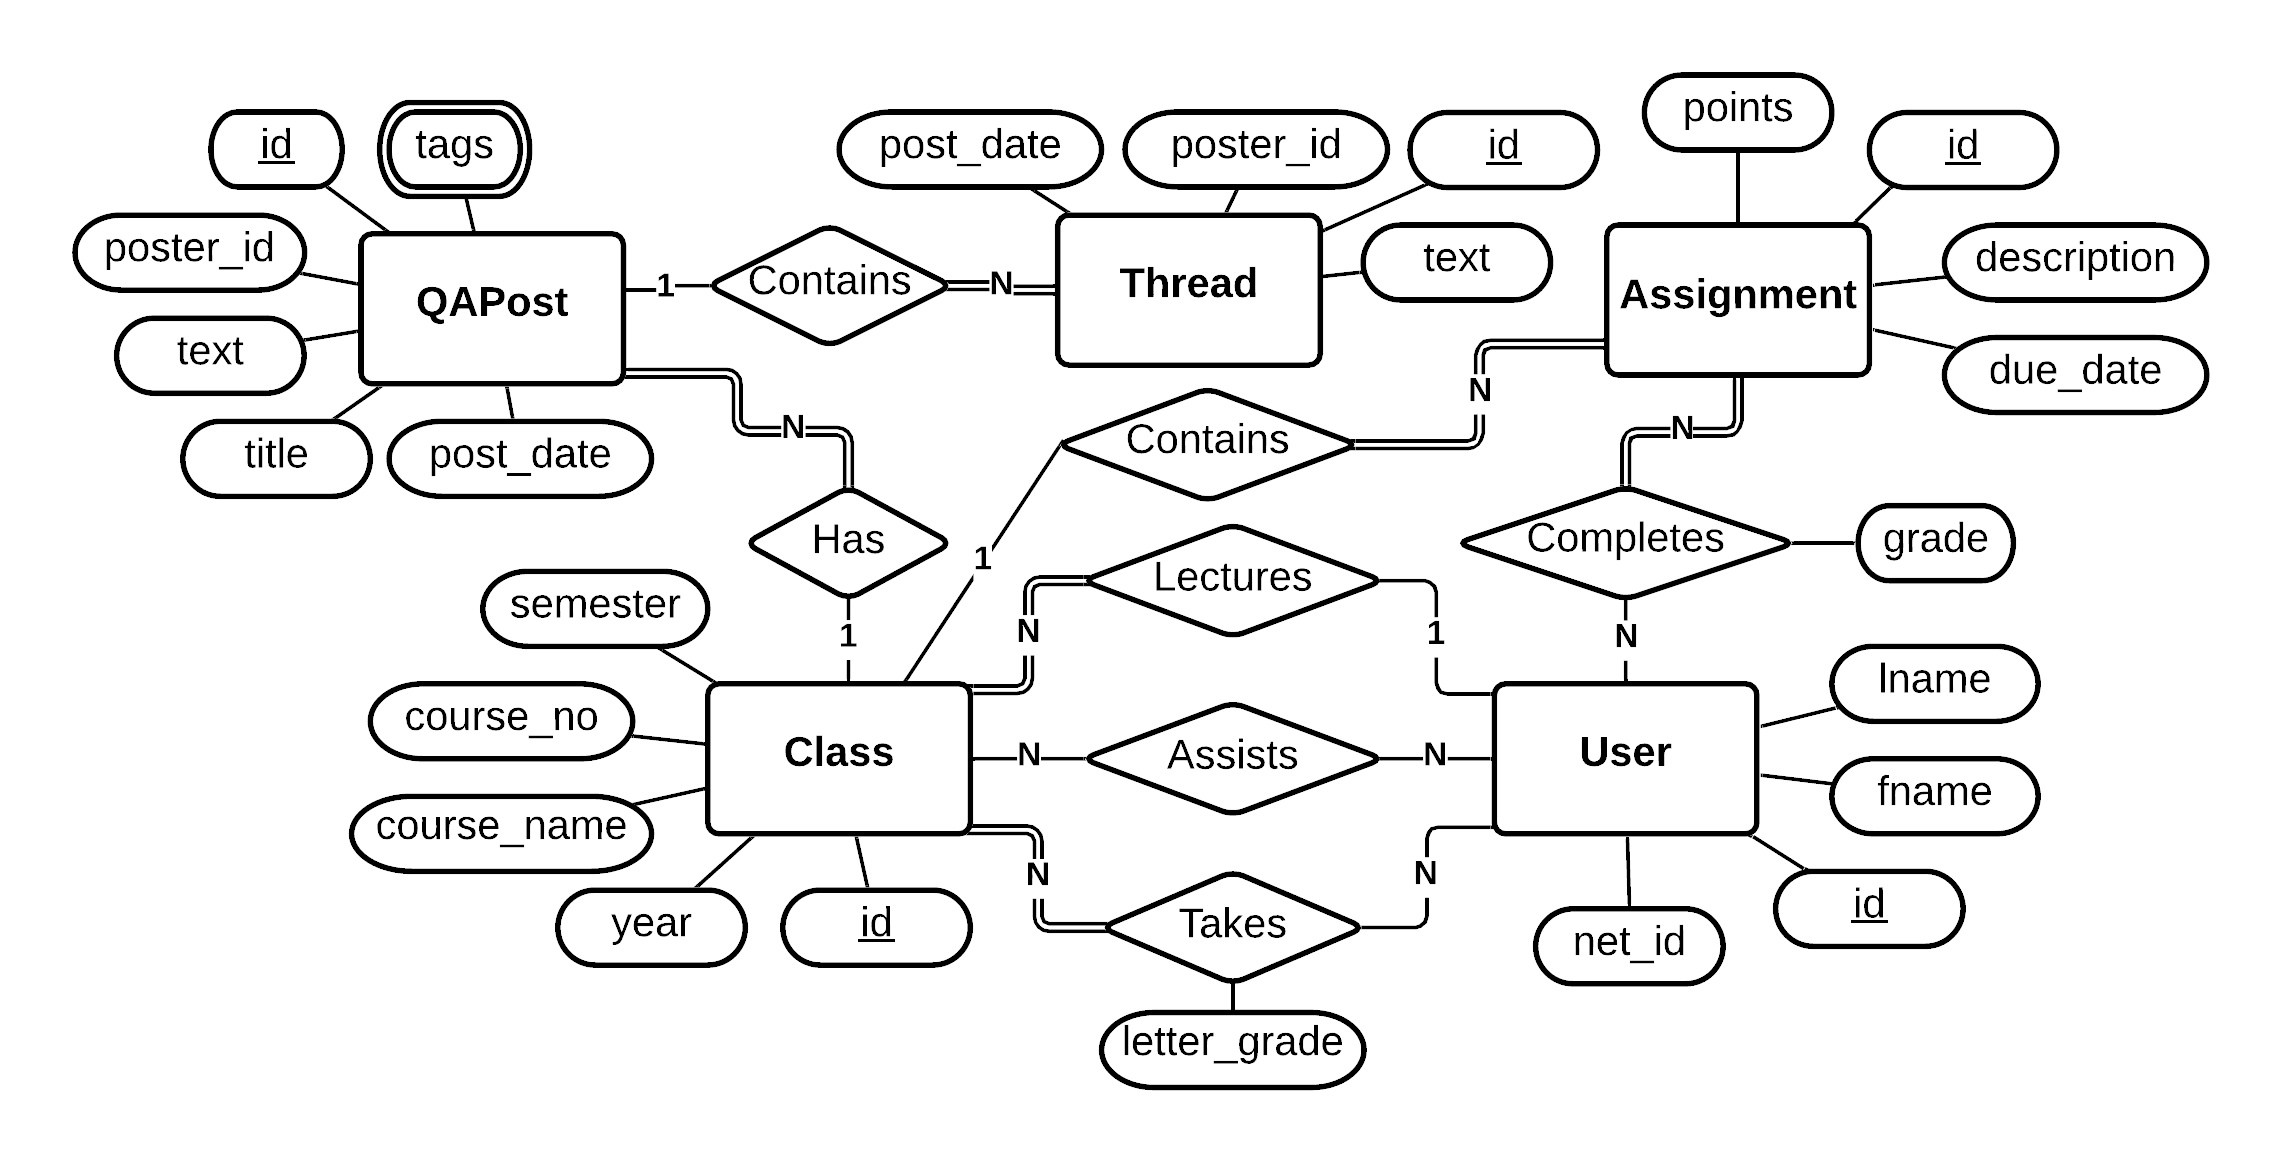
\includegraphics[scale=0.131]{er_diagram.png}
	\end{center}
	
	\section{Relational Model Creation}
	
	The initial relational model consists of the following relations:
	\begin{itemize}
		\item User(\underline{id}, net\_id, fname, lname)
		\item Class(\underline{id}, course\_no, course\_name, semester, year, lecturer\_id$\to$User.id)
		\item Assignment(\underline{id}, name, due\_date, description, points, class\_id$\to$Class.id)
		\item QAPost(\underline{id}, title, post\_date, text, poster\_id$\to$User.id,  class\_id$\to$Class.id)
		\item Thread(\underline{id}, post\_date, text, poster\_id$\to$User.id, parent\_id$\to$QAPost.id)
		\item Tags(\underline{post\_id}$\to$QAPost.id, \underline{tag})
		\item Takes(\underline{user\_id}$\to$User.id, \underline{class\_id}$\to$Class.id, letter\_grade)
		\item Completes(\underline{user\_id}$\to$User.id, \underline{assignment\_id}$\to$Assignment.id, grade)
		\item Assists(\underline{user\_id}$\to$User.id, \underline{class\_id}$\to$Class.id)
	\end{itemize}
	
	\section{Database Normalization}
	To ensure that the database conforms to 3NF, start by ensuring that the relation schema is in 1NF, which states that
	\begin{itemize}
		\item Every attribute in the relational model has atomic values.
	\end{itemize}
	By this rule, the relation schema is already in 1NF. 2NF states that
	\begin{itemize}
		\item 1NF is satisfied, and
		\item Non-candidate-key attributes are not partially dependent on any key of the relation, i.e., every non-key attribute is fully functionally dependent on the primary key.
	\end{itemize}
	Since the relation schema is already in 1NF, I argue the second point of the 2NF constraints: none of the non-key attributes are partially dependent on their respective relation's primary key. This can be seen readily where the primary key is a single element, and for those relations that contain a key with  size greater than 1, there are only one or no non-key attribute.\\\\
	Now, to convert to 3NF, its constraints must include that
	\begin{itemize}
		\item 2NF is satisfied, and
		\item Every non-key attribute is non-transitively dependent on all the keys.
	\end{itemize}
	I argue that the relational model proposed above satisfies the 3NF conditions, as no non-key attribute in any of the relations is dependent on another non-key attribute in that same relation.\\\\
	With the satisfaction of 3NF conditions, the normalization of the database is considered complete.
	
	\section{Data Description}
	All of the \verb|.csv| files are generated using the \verb|extract.py| script and some further manual tweaking on the data source files \verb|canvas.csv| and \verb|qa.csv|. There may exist some slight differences in data due to manual corrections.\\
	For a more graphical view, please see section 6 (``Data Diagram'').
	\begin{center}
		\begin{tabular}{c | c | l}
			\toprule
			\multicolumn{3}{c}{\textbf{Table user}} \\
			\multicolumn{3}{c}{Defines all existing users in Canvas.}\\
			\midrule
			Attribute Name & Attribute Type & \multicolumn{1}{c}{Description} \\
			\verb|id| & \verb|CHAR(10)| & Personal ID for the user. (PK)\\
			\verb|net_id| & \verb|VARCHAR(64)| & NetID used for login. \\
			\verb|fname| & \verb|TINYTEXT| & First name of the user. \\
			\verb|lname| & \verb|TINYTEXT| & Last name of the user. \\
			\bottomrule
		\end{tabular}\vspace{1.5em}
	
		\begin{tabular}{c | c | l}
			\toprule
			\multicolumn{3}{c}{\textbf{Table class}} \\
			\multicolumn{3}{c}{Defines all classes that exists in Canvas.}\\
			\midrule
			Attribute Name & Attribute Type & \multicolumn{1}{c}{Description} \\
			\verb|id| & \verb|CHAR(10)| & Unique identifier for the class. (PK)\\
			\verb|course_no| & \verb|VARCHAR(8)| & Course number (e.g., CS377) for the class.\\
			\verb|course_name| & \verb|TINYTEXT| & Course name (e.g., Database Systems) for the class.\\
			\verb|semester| & \verb|VARCHAR(6)| & Semester the course is offered in.\\
			\verb|year| & \verb|INT| & Year the course is offered in.\\
			\verb|lecturer_id| & \verb|CHAR(10)| & The personal ID for the teaching professor. (FK$\to$user.id)\\
			\bottomrule
		\end{tabular}\vspace{1.5em}

		\begin{tabular}{c | c | l}
			\toprule
			\multicolumn{3}{c}{\textbf{Table assignment}} \\
			\multicolumn{3}{c}{Defines all assignments that exists in Canvas.}\\
			\midrule
			Attribute Name & Attribute Type & \multicolumn{1}{c}{Description} \\
			\verb|id| & \verb|CHAR(10)| & Unique identifier for the assignment. (PK)\\
			\verb|name| & \verb|VARCHAR(64)| & Name of the assignment.\\
			\verb|due_date| & \verb|TIMESTAMP| & Due date of the assignment.\\
			\verb|description| & \verb|TEXT| & Detailed description of the assignment.\\
			\verb|points| & \verb|INT| & Maximum amount of points achievable.\\
			\verb|class_id| & \verb|CHAR(10)| & The class ID that this assignment belongs to. (FK$\to$class.id)\\
			\bottomrule
		\end{tabular}\vspace{1.5em}
		
		\begin{tabular}{c | c | l}
			\toprule
			\multicolumn{3}{c}{\textbf{Table qapost}} \\
			\multicolumn{3}{c}{Defines all Q\&A posts that exists in the Q\&A Corner.}\\
			\midrule
			Attribute Name & Attribute Type & \multicolumn{1}{c}{Description} \\
			\verb|id| & \verb|CHAR(10)| & Unique identifier for the Q\&A post. (PK)\\
			\verb|title| & \verb|TINYTEXT| & The title of the Q\&A post. \\
			\verb|post_date| & \verb|TIMESTAMP| & The date when this Q\&A post was posted. \\
			\verb|text| & \verb|TEXT| & The body of the Q\&A post. \\
			\verb|poster_id| & \verb|CHAR(10)| & The personal ID of the poster. (FK$\to$user.id) \\
			\verb|class_id| & \verb|CHAR(10)| & The class ID that this Q\&A post belongs to. (FK$\to$class.id) \\
			\bottomrule
		\end{tabular}\vspace{1.5em}
			
		\begin{tabular}{c | c | l}
			\toprule
			\multicolumn{3}{c}{\textbf{Table thread}} \\
			\multicolumn{3}{c}{Defines all non-parent posts in the Q\&A Corner.}\\
			\midrule
			Attribute Name & Attribute Type & \multicolumn{1}{c}{Description} \\
			\verb|id| & \verb|CHAR(10)| & Unique identifier for the thread post. (PK) \\
			\verb|post_date| & \verb|TIMESTAMP| & The date when this thread post was posted.\\
			\verb|text| & \verb|TEXT| & The body of the thread post.\\
			\verb|poster_id| & \verb|CHAR(10)| & The personal ID of the poster. (FK$\to$user.id)\\
			\verb|parent_id| & \verb|CHAR(10)| & The Q\&A post ID that this thread post belongs to.\\
			& & (FK$\to$qapost.id)\\
			\bottomrule
		\end{tabular}\vspace{1.5em}
			
		\begin{tabular}{c | c | l}
			\toprule
			\multicolumn{3}{c}{\textbf{Table tags}} \\
			\multicolumn{3}{c}{Defines all tags associated with posts in the Q\&A Corner.}\\
			\midrule
			Attribute Name & Attribute Type & \multicolumn{1}{c}{Description} \\
			\verb|post_id| & \verb|CHAR(10)| & The Q\&A post's ID. (FK$\to$qapost.id)\\
			\verb|tag| & \verb|VARCHAR(32)| & A tag that the post contains.\\
			\bottomrule
		\end{tabular}\vspace{1.5em}
			
		\begin{tabular}{c | c | l}
			\toprule
			\multicolumn{3}{c}{\textbf{Table takes}} \\
			\multicolumn{3}{c}{Defines all student-taking-class relationships, and their letter grades in Canvas.}\\
			\midrule
			Attribute Name & Attribute Type & \multicolumn{1}{c}{Description} \\
			\verb|user_id| & \verb|CHAR(10)| & Student's personal ID. (PK, FK$\to$user.id) \\
			\verb|class_id| & \verb|CHAR(10)| & Class's unique ID. (PK, FK$\to$class.id) \\
			\verb|letter_grade| & \verb|VARCHAR(3)| & Letter grade the student obtained for class.\\
			\bottomrule
		\end{tabular}\vspace{1.5em}
			
		\begin{tabular}{c | c | l}
			\toprule
			\multicolumn{3}{c}{\textbf{Table completes}} \\
			\multicolumn{3}{c}{Defines all student-completing-assignment relationships, and their numeric grades in Canvas.}\\
			\midrule
			Attribute Name & Attribute Type & \multicolumn{1}{c}{Description} \\
			\verb|user_id| & \verb|CHAR(10)| & Student's personal ID. (PK, FK$\to$user.id) \\
			\verb|assignment_id| & \verb|CHAR(10)| & Assignment's unique ID. (PK, FK$\to$assignment.id) \\
			\verb|grade| & \verb|VARCHAR(4)| & Grade the student obtained on assignment. \\
			\bottomrule
		\end{tabular}\vspace{1.5em}
	
		\begin{tabular}{c | c | l}
			\toprule
			\multicolumn{3}{c}{\textbf{Table assists}} \\
			\multicolumn{3}{c}{Defines all TA-assists-class relationships.}\\
			\midrule
			Attribute Name & Attribute Type & \multicolumn{1}{c}{Description} \\
			\verb|user_id| & \verb|CHAR(10)| & TA's personal ID. (PK, FK$\to$user.id)\\
			\verb|class_id| & \verb|CHAR(10)| & ID of the class being assisted. (PK, FK$\to$class.id) \\
			\bottomrule
		\end{tabular}

	\end{center}

	\section{Data Diagram}
	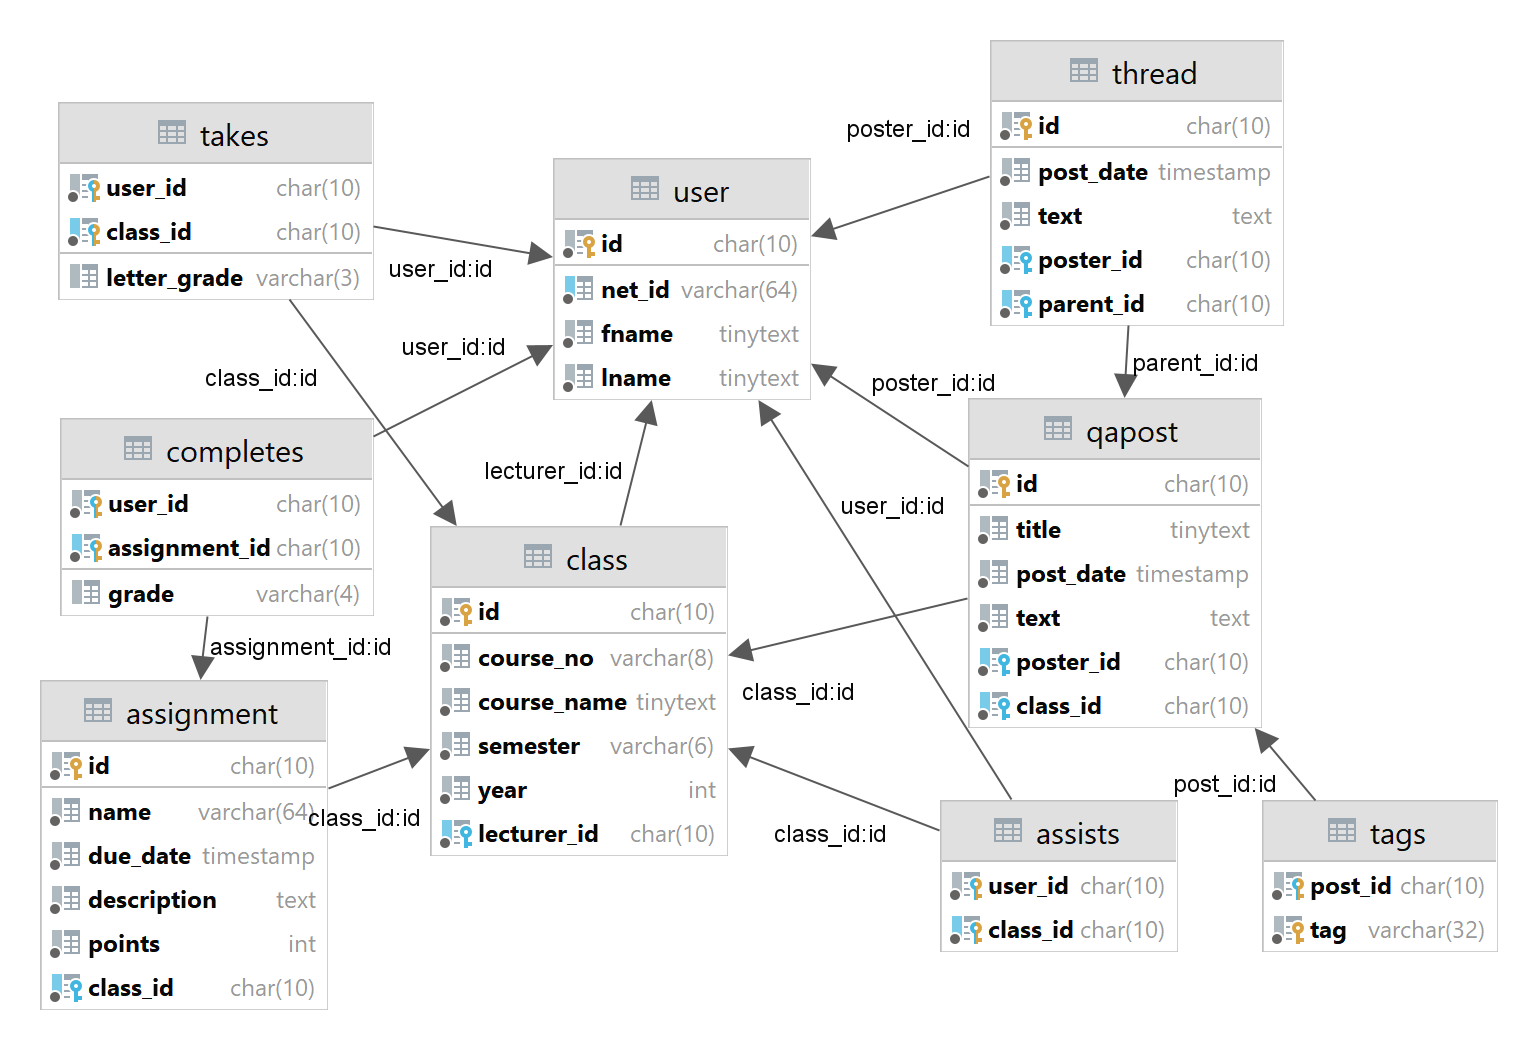
\includegraphics[scale=0.3]{canvas_db.png}
	
	\section{Project File Directory}
	\begin{center}
		\begin{tabular}{ r | l }
			\toprule
			\multicolumn{2}{c}{\textbf{File Directory}} \\
			\midrule
				\verb|cs377-course-project/| & Project root \\
				\verb|index.php| & Login page (Q10) \\
				\verb|home.php| & Home page (Q10) \\
				\verb|view_course.php| & Course view page (Q7, Q8) \\
				\verb|create_assignment.php| & Assignment creation page (Q8) \\
				\verb|qa_posts.php| & Q\&A posts page (Q9) \\
				\verb|view_thread.php| & Single post view page (Q9) \\
				\verb|transcript.php| & Transcript view page (Q11) \\
				\verb|helpers.php| & Helper functions file \\
				\verb|logout.php| & Logout redirect page \\
				\verb|README.txt| & Honor code file \\
				\verb|er_diagram.png| & ER diagram used in Section 2 (``ER Design'')\\
				\verb|canvas_db.png| & Database diagram used in Section 6 (``Data Diagram'')\\
				\verb|extract.py| & Python extraction helper script \\
				\verb|report.pdf| & This report \\
				\verb|*.sql| & SQL database setup/teardown scripts \\
				\verb|*.csv| & Table data files \\
			\bottomrule
		\end{tabular}
	\end{center}
	
	\section{Closing Remarks and Error Handling}
	\begin{itemize}
		\item My personal Google Cloud compute instance can be found at \url{http://jerry.games/377}.
		\item Please, do \emph{not} run the \verb|extract.py| file. It will corrupt all exported \verb|csv| data. Feel free to take a look inside however.
		\item There is a small chance that I have left my personal compute instance's address as a database connection argument. If you find your data failing to update on the local server, please navigate to the project root and execute \verb|sed -i 's/jerry.games/localhost/g' *| to replace all occurrences of \verb|jerry.games| with \verb|localhost|.
		\item A lot of fields do not have error checking for apostrophes. Avoid entering apostrophes if errors occur.
	\end{itemize}
	
	\clearpage
	
\end{document}